% Results and Analysis slides

\begin{frame}{Méthodologie de comparaison}
    \begin{itemize}
        \item \textbf{Comparaison systématique RK4 vs Parareal}
        \item \textbf{Aspects analysés :}
        \begin{itemize}
            \item Évolution temporelle (X, Y, Z)
            \item Erreur absolue entre solutions
            \item Convergence vers états stationnaires/attracteurs
            \item Portraits de phase
        \end{itemize}
        \item \textbf{Régimes étudiés :} $\tau = 0.5$, $2.0$, $5.0$
    \end{itemize}
\end{frame}

\begin{frame}{Régime non-marcheur ($\tau = 0.5$)}
    \begin{columns}
        \column{0.6\textwidth}
        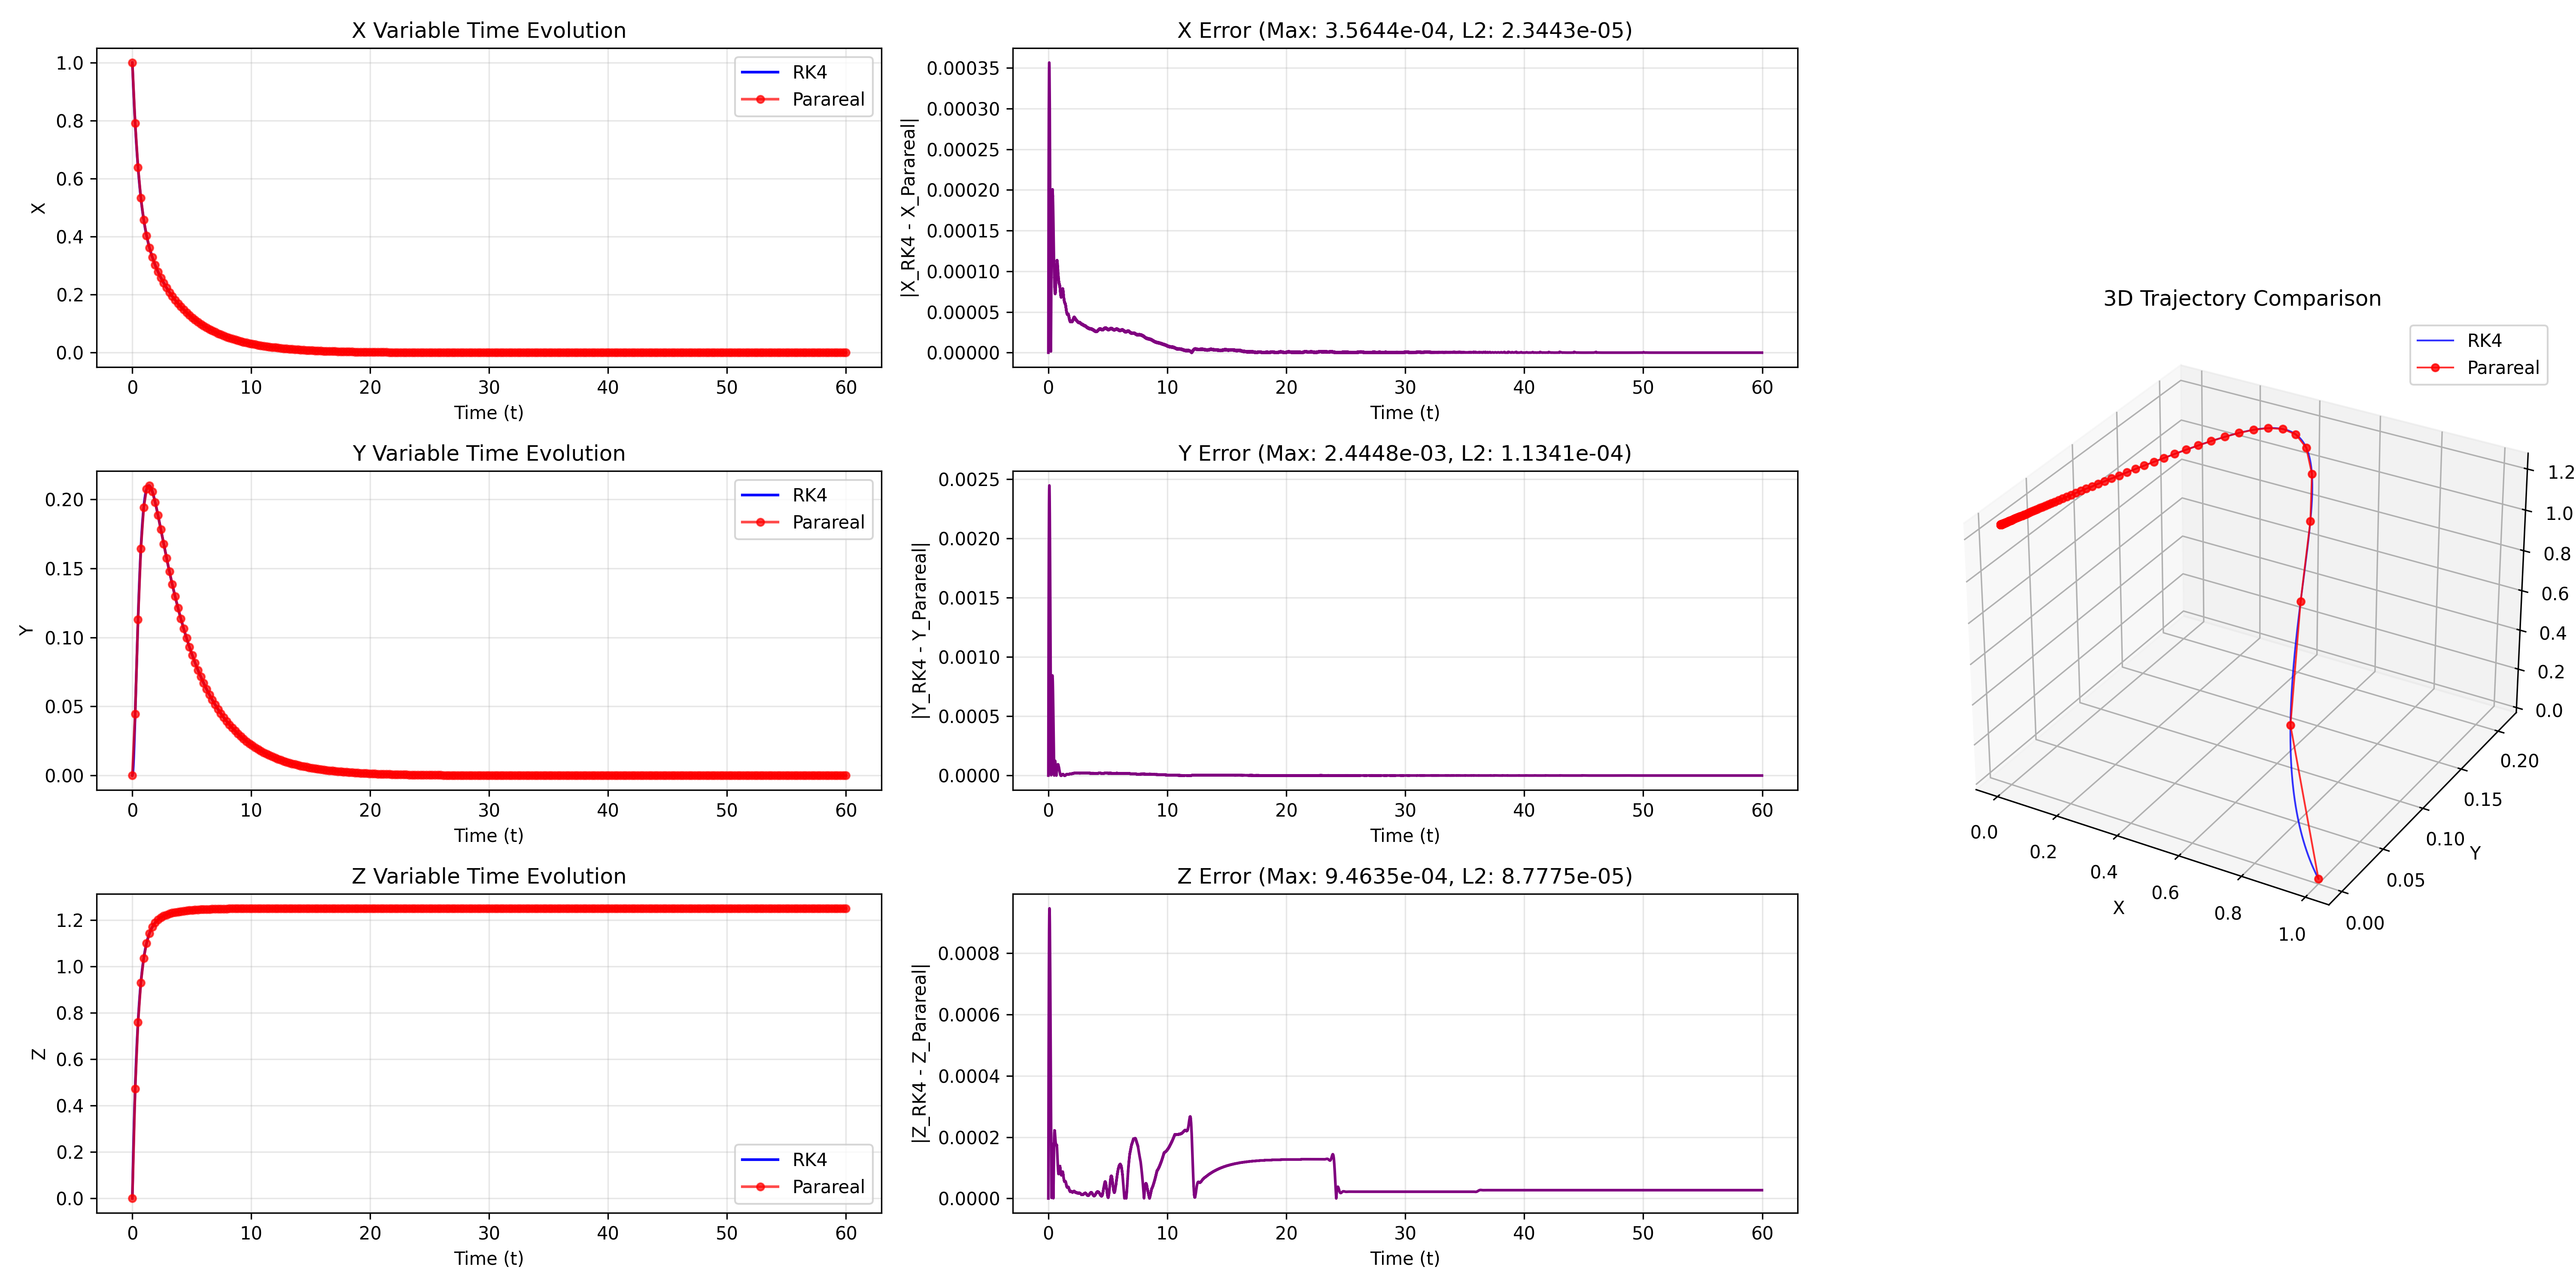
\includegraphics[width=\textwidth]{../Document/figures/comparisons/comparison_tau0.5_comparison}
        
        \column{0.4\textwidth}
        \textbf{Observations :}
        \begin{itemize}
            \item Excellente concordance
            \item Erreurs $< 10^{-6}$
            \item Stabilité numérique
        \end{itemize}
    \end{columns}
\end{frame}

\begin{frame}{Marche régulière ($\tau = 2.0$)}
    \begin{columns}
        \column{0.6\textwidth}
        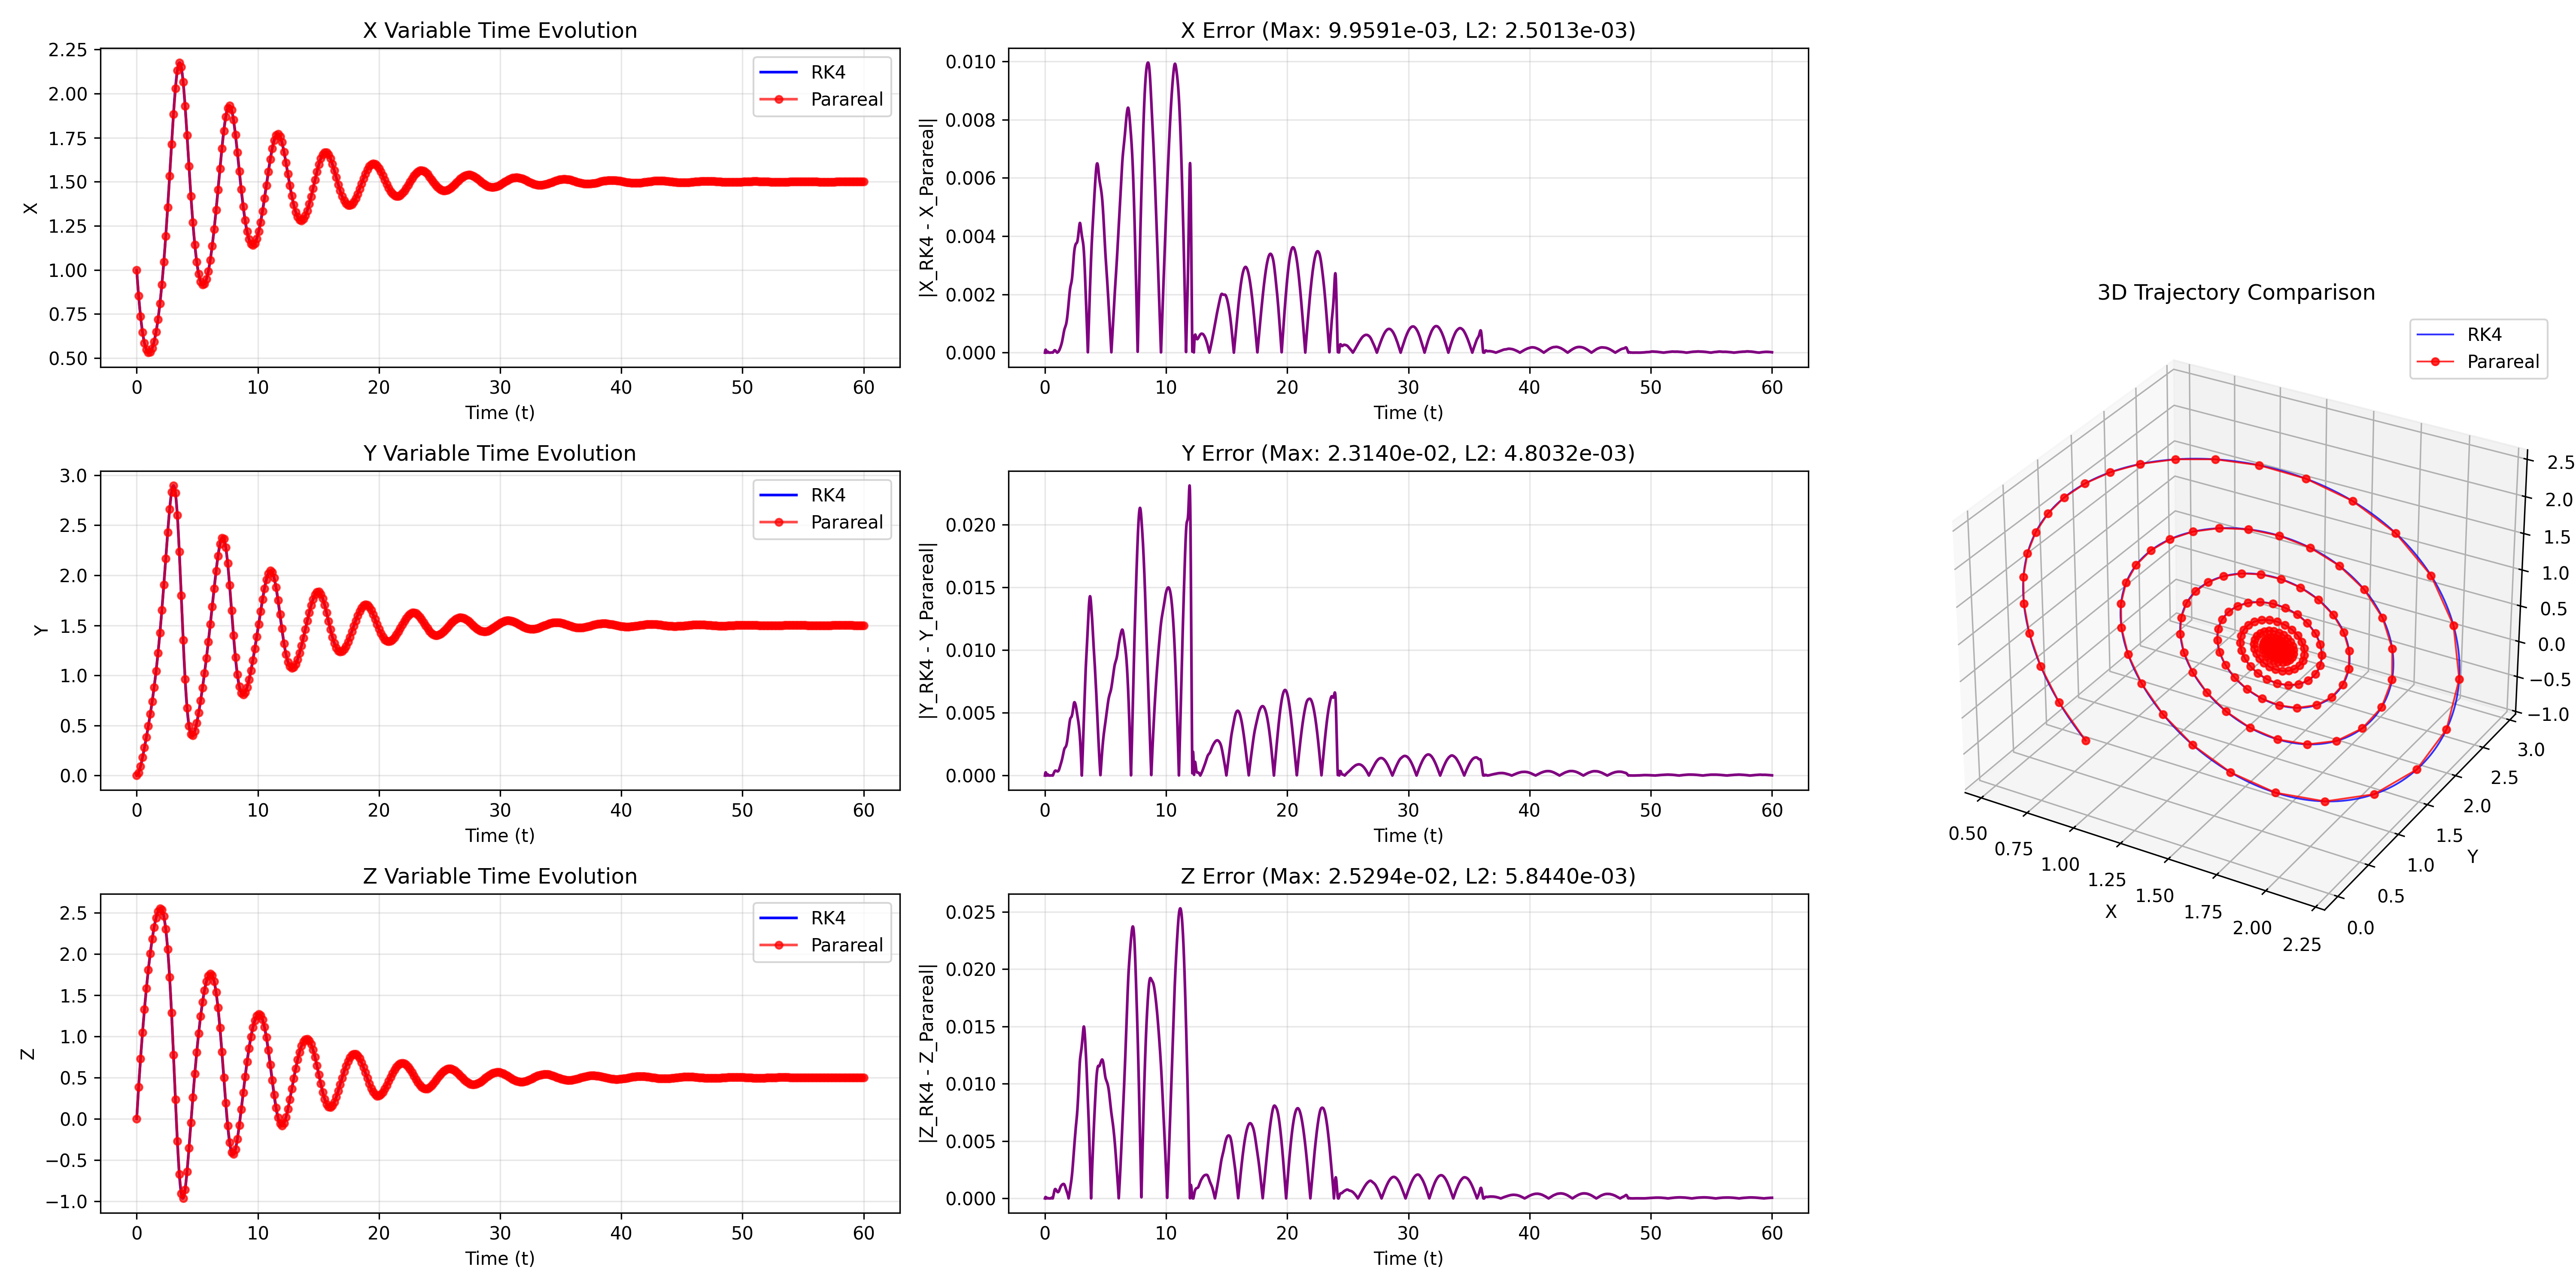
\includegraphics[width=\textwidth]{../Document/figures/comparisons/comparison_tau2.0_comparison}
        
        \column{0.4\textwidth}
        \textbf{Résultats :}
        \begin{itemize}
            \item États stationnaires fidèles
            \item Stabilisation rapide
            \item Précision maintenue
        \end{itemize}
    \end{columns}
\end{frame}

\begin{frame}{Régime chaotique ($\tau = 5.0$)}
    \begin{columns}
        \column{0.6\textwidth}
        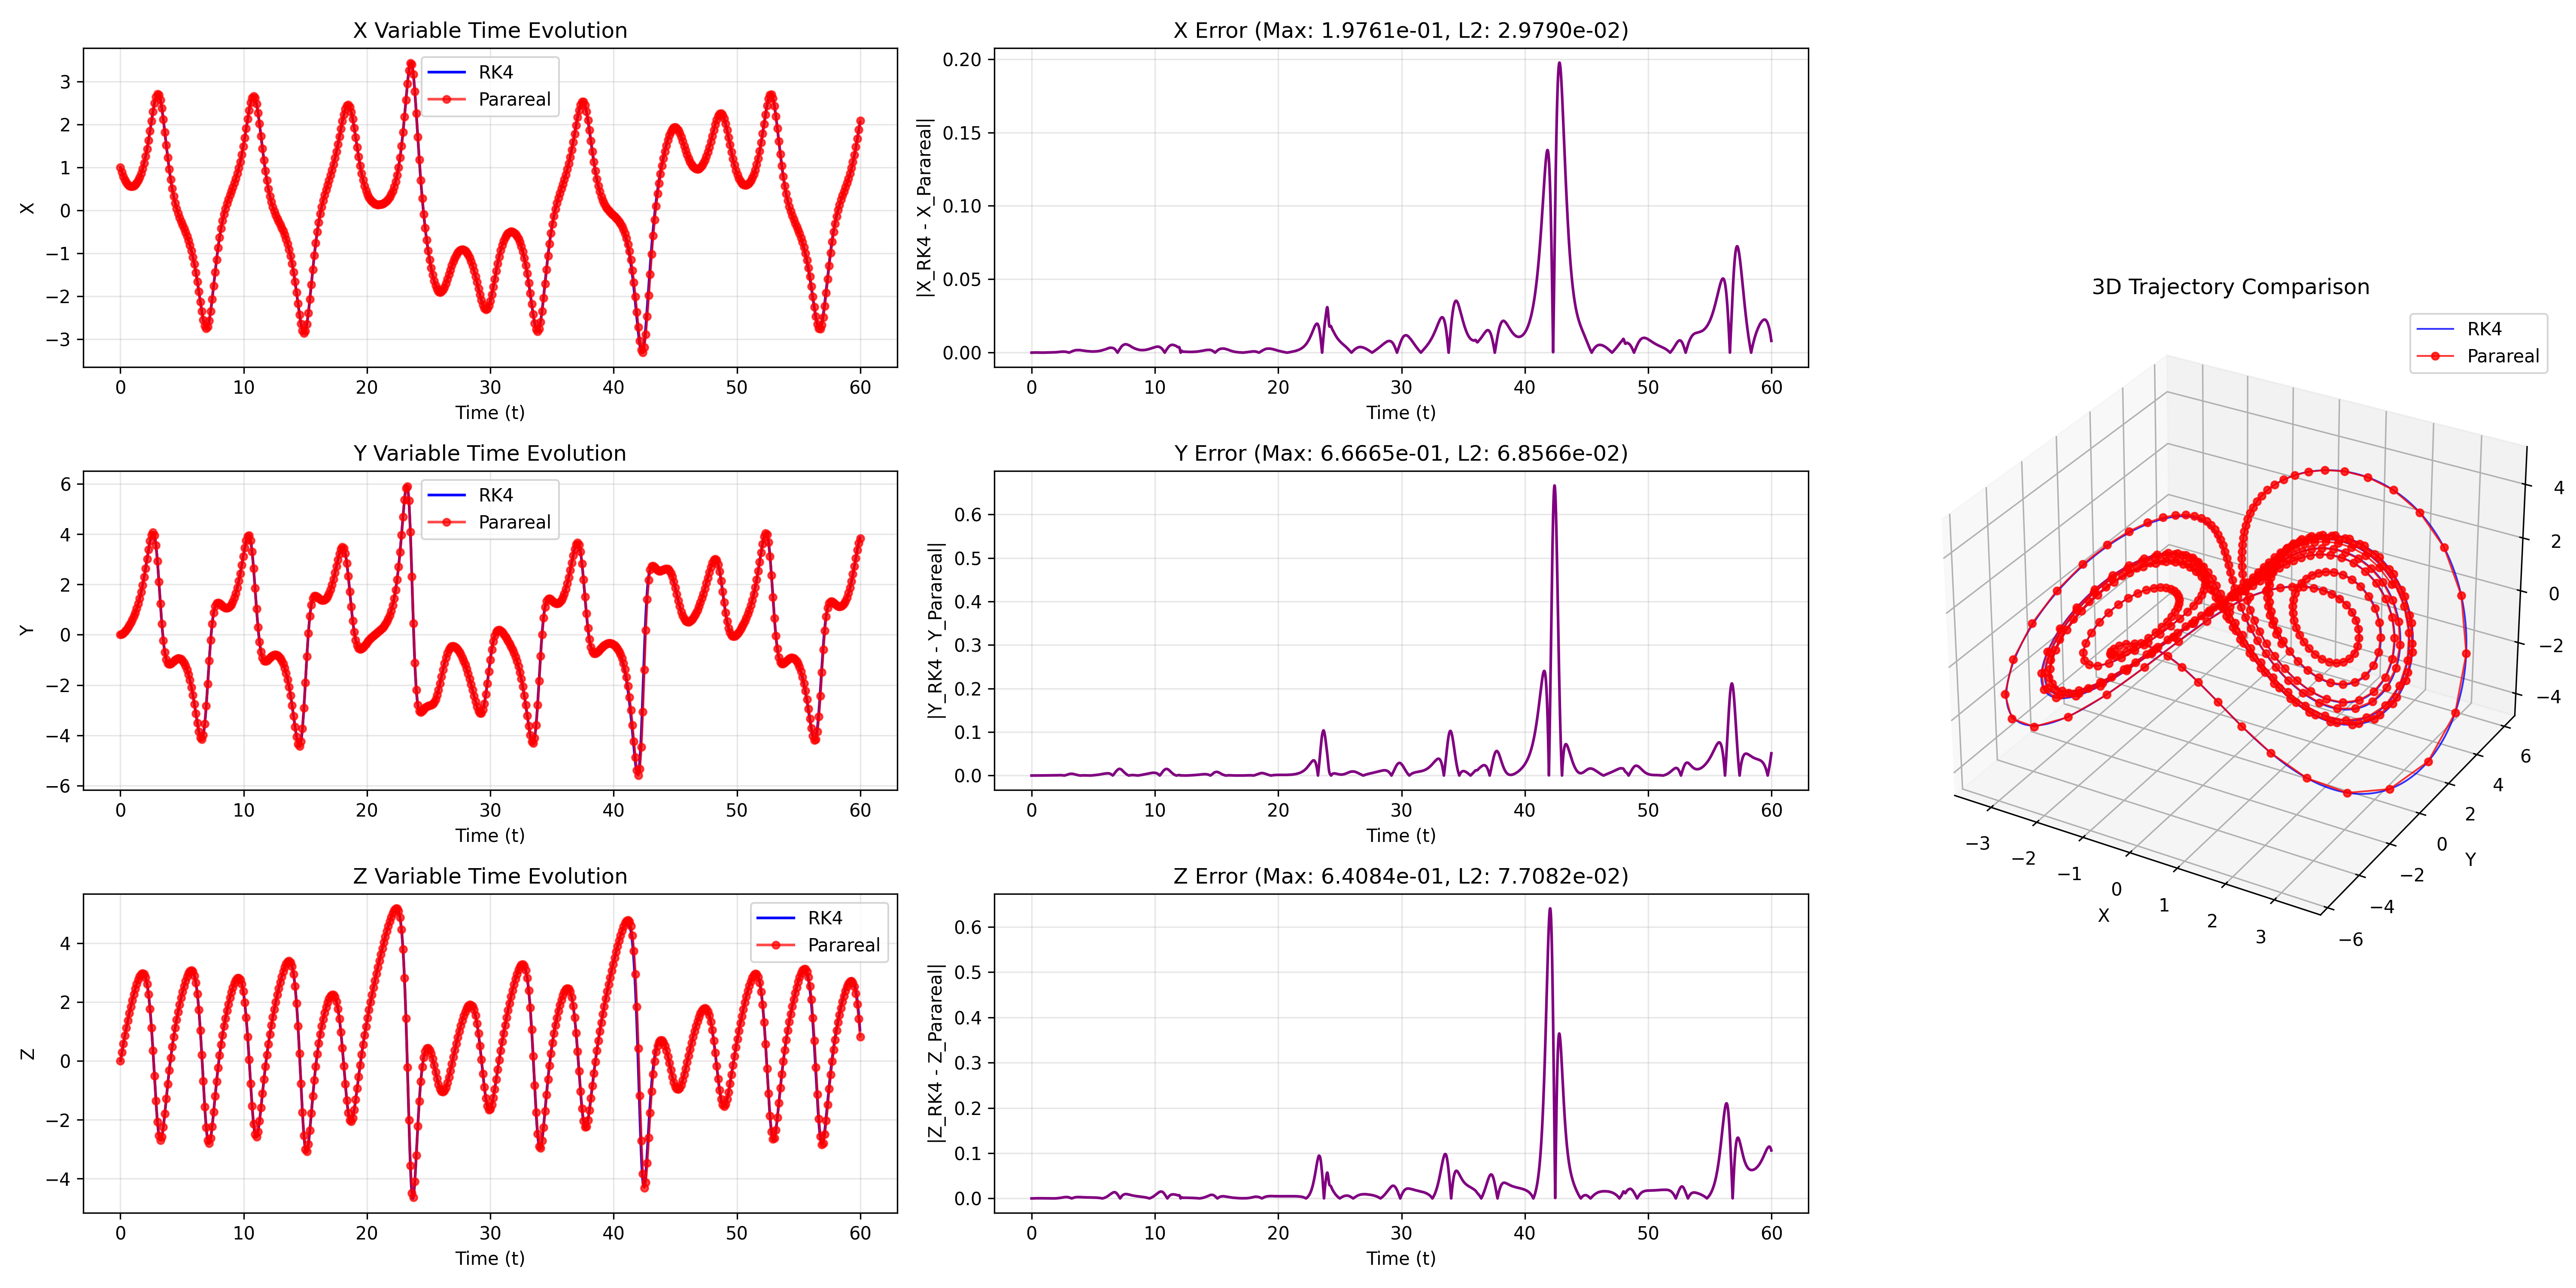
\includegraphics[width=\textwidth]{../Document/figures/comparisons/comparison_tau5.0_comparison}
        
        \column{0.4\textwidth}
        \textbf{Analyse :}
        \begin{itemize}
            \item Cohérence des trajectoires
            \item Pics d'erreur aux transitions
            \item Structure d'attracteur préservée
        \end{itemize}
    \end{columns}
\end{frame}

\begin{frame}{Performances temporelles}
    \begin{columns}
        \column{0.5\textwidth}
        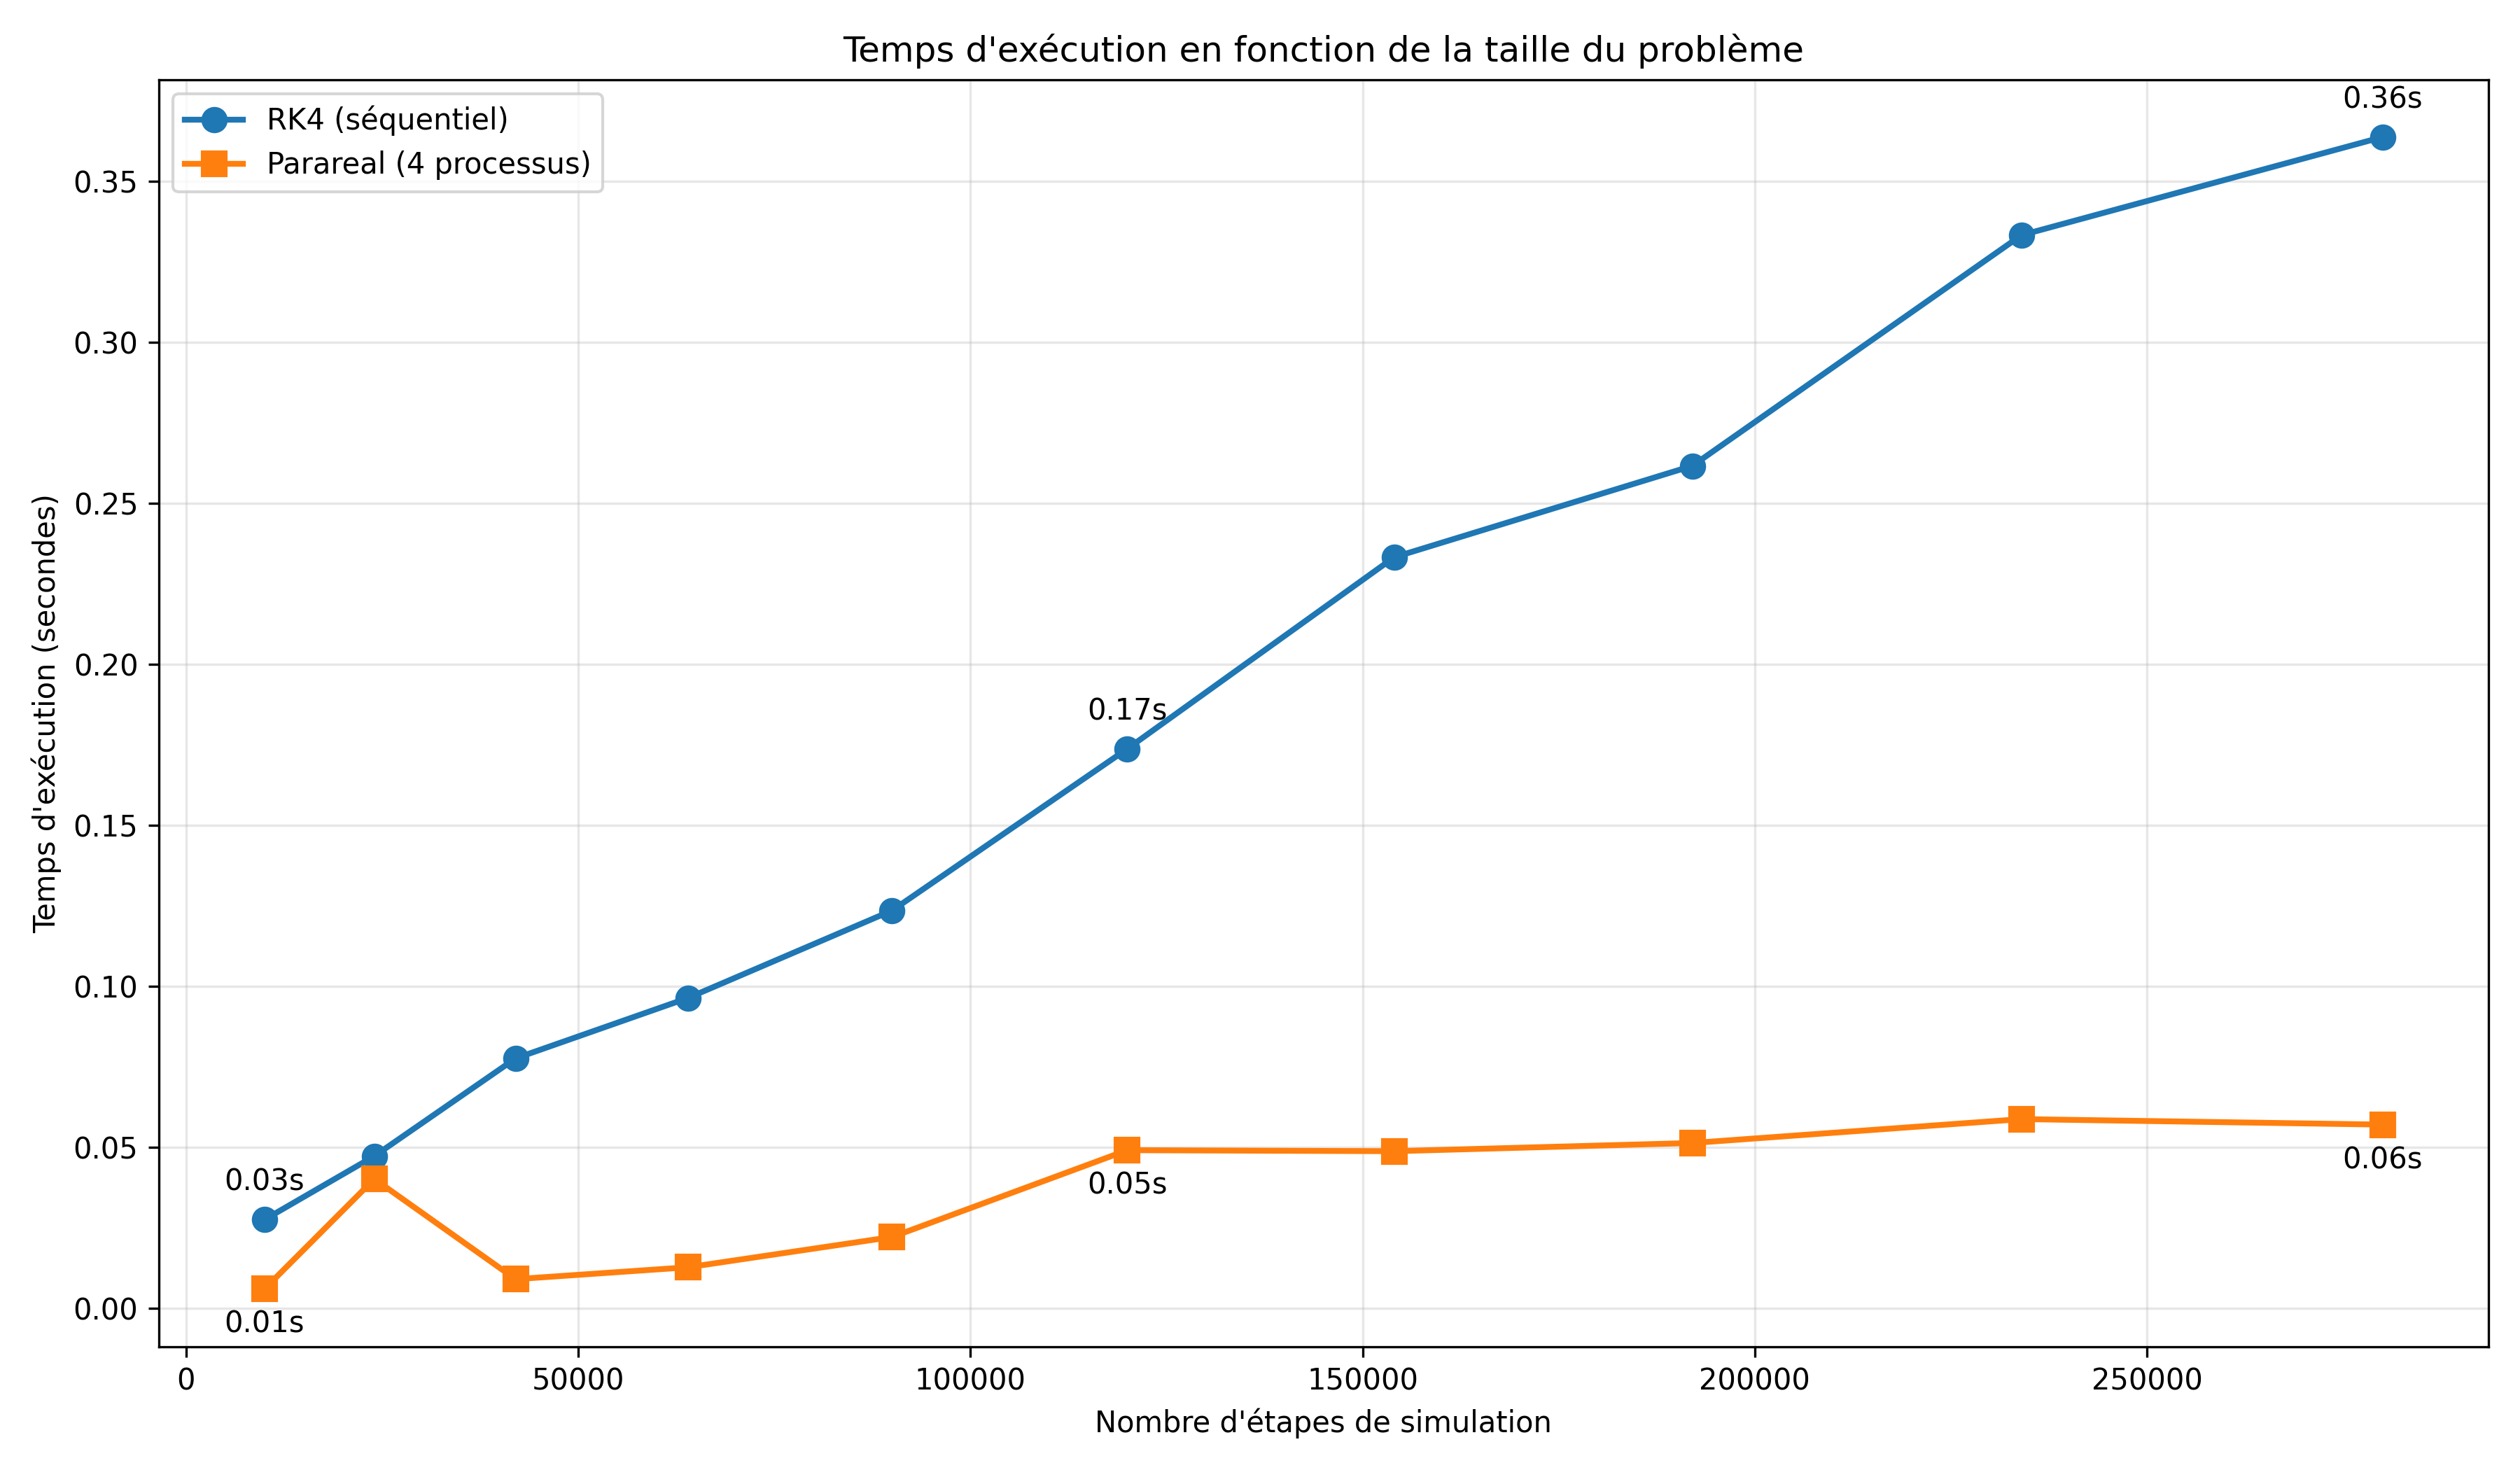
\includegraphics[width=\textwidth]{../Document/figures/benchmarks/execution_time_steps}
        \textbf{Temps d'exécution}
        
        \column{0.5\textwidth}
        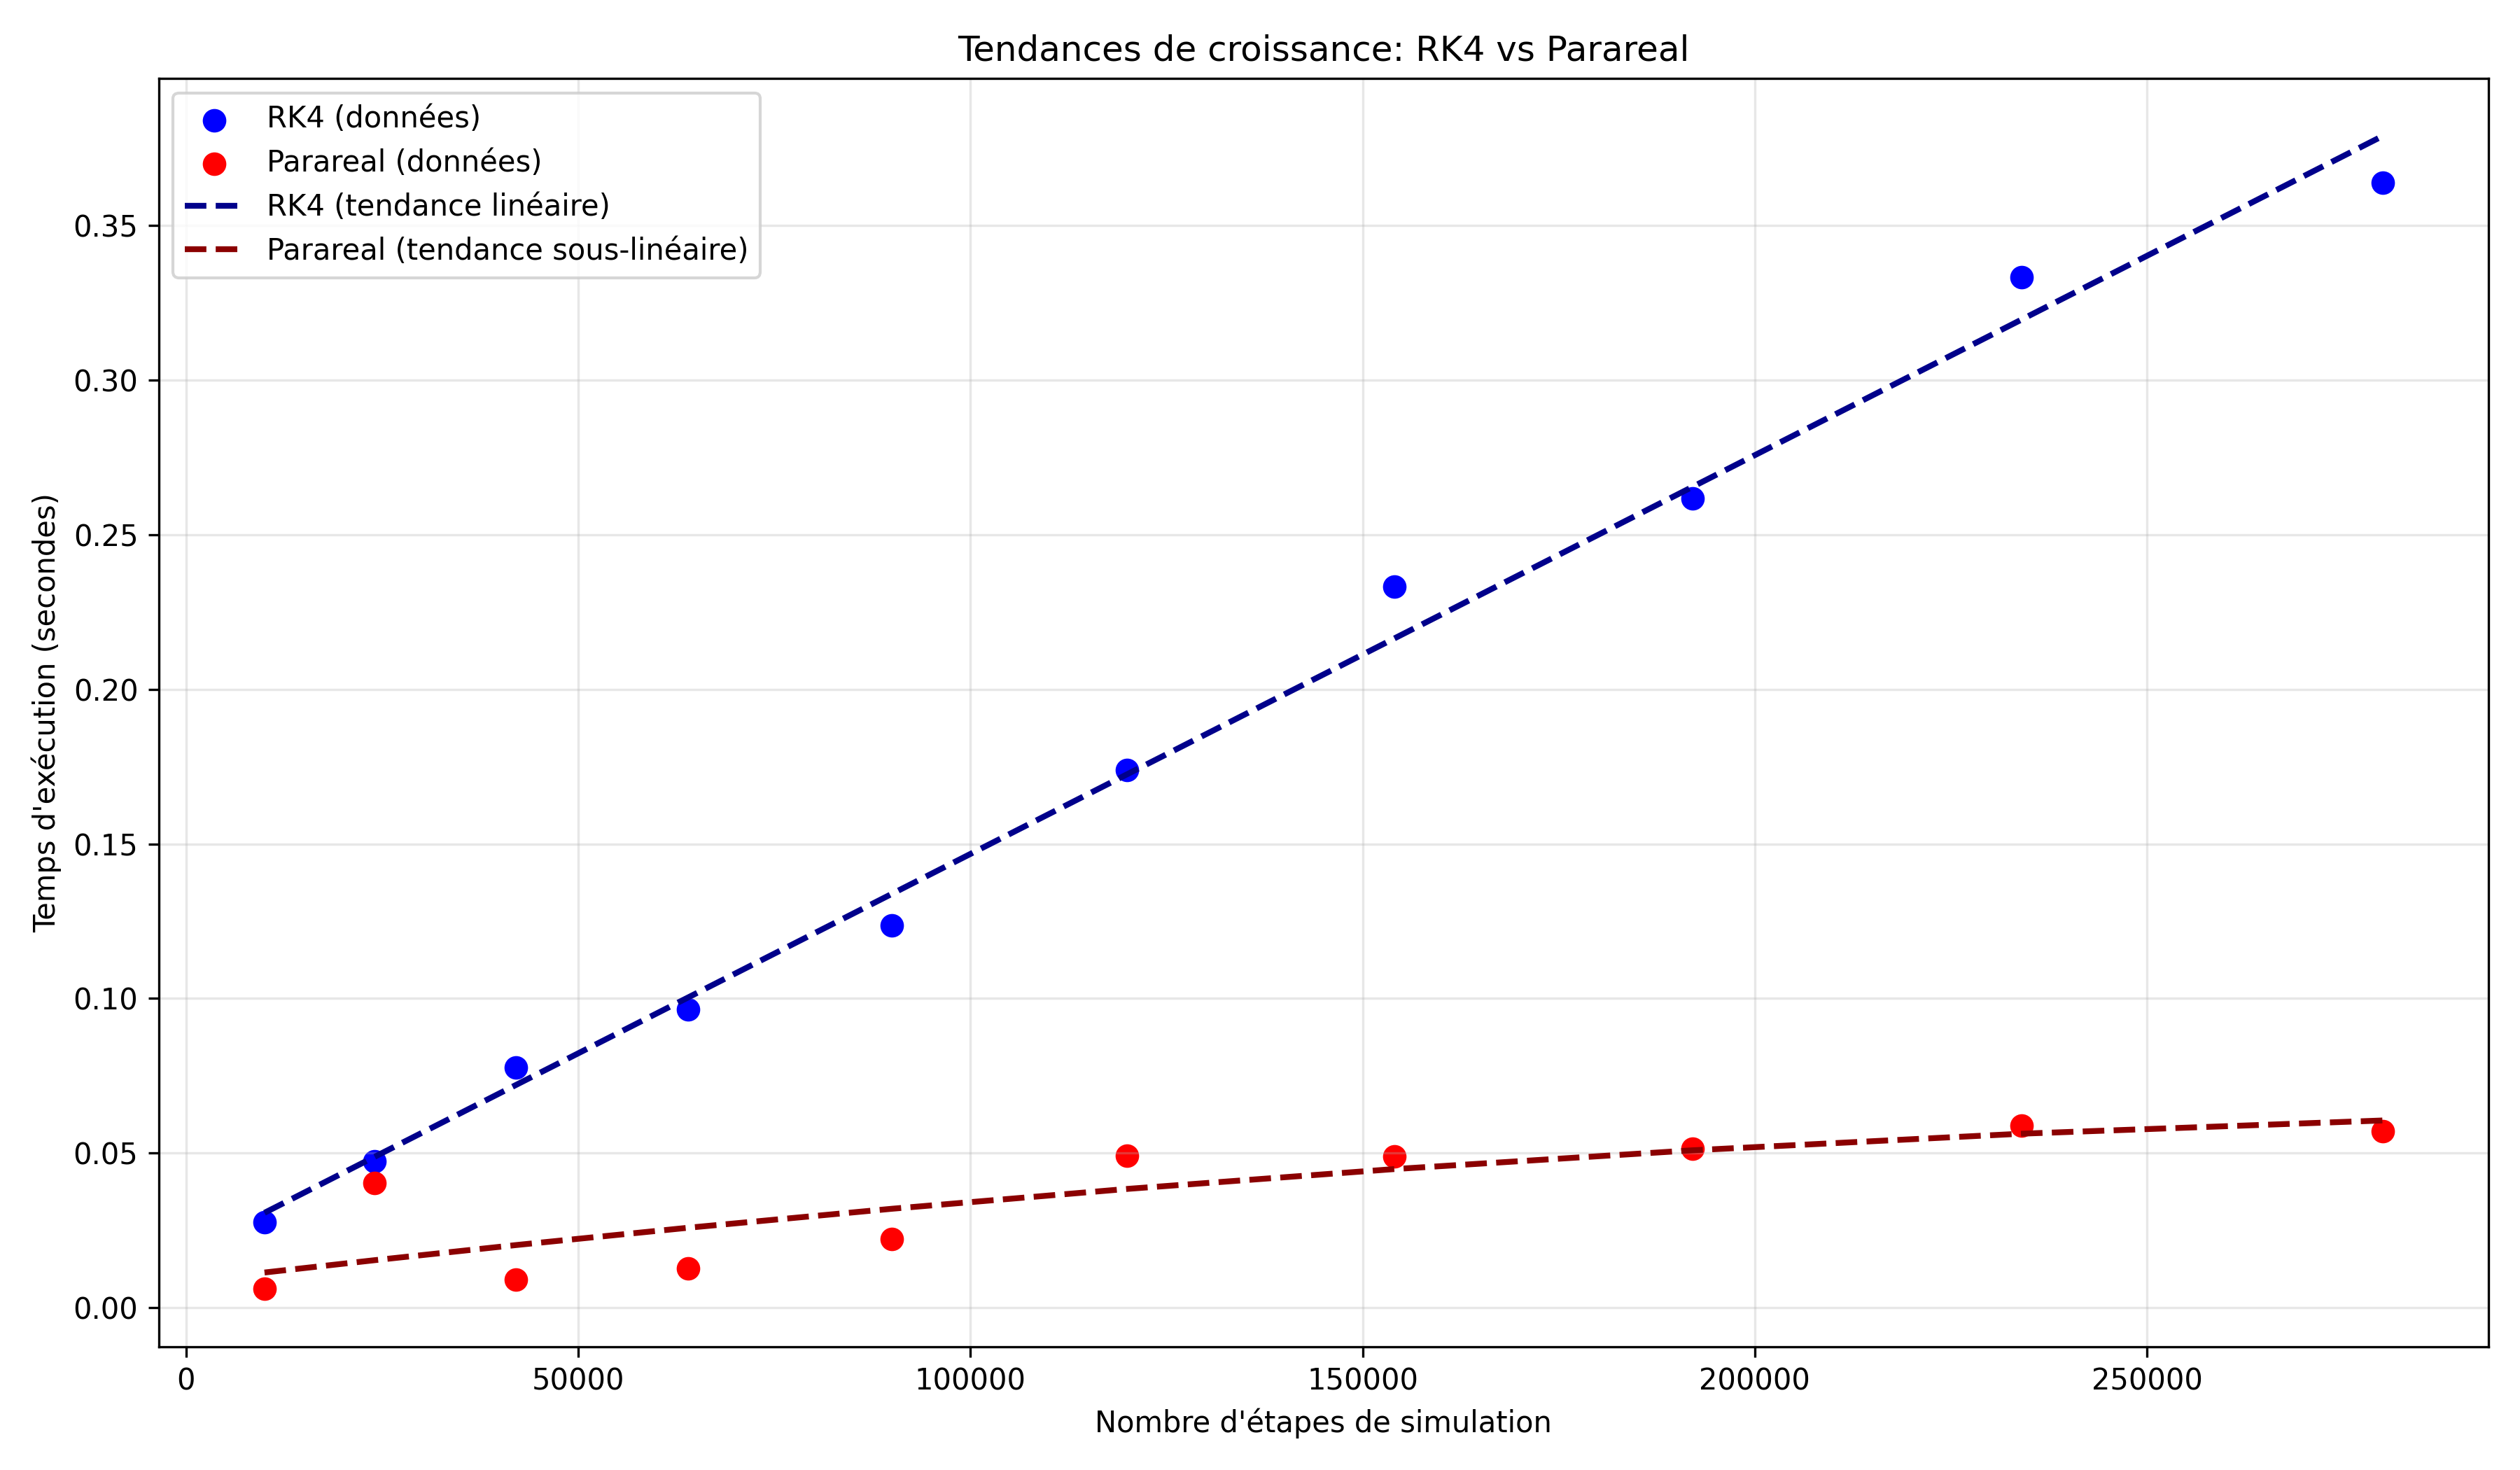
\includegraphics[width=\textwidth]{../Document/figures/benchmarks/growth_trends}
        \textbf{Tendances de croissance}
    \end{columns}
    \vspace{0.3cm}
    \begin{itemize}
        \item Gain significatif en temps de calcul
        \item Efficacité > 50\% à grande échelle
        \item Scalabilité quasi-linéaire jusqu'à 250000 itérations
    \end{itemize}
\end{frame}

\begin{frame}{Synthèse des performances}
    \begin{itemize}
        \item \textbf{Précision}
        \begin{itemize}
            \item Erreurs relatives < $10^{-4}$ (régimes stables)
            \item Conservation des caractéristiques qualitatives
            \item Préservation des invariants
        \end{itemize}
        \vspace{0.3cm}
        \item \textbf{Stabilité}
        \begin{itemize}
            \item Robustesse dans tous les régimes
            \item Gestion efficace des transitions
            \item Contrôle des erreurs numériques
        \end{itemize}
    \end{itemize}
\end{frame}